%-----------------------------------------------------------------------------------------------------------------------------------------------%
%	The MIT License (MIT)
%
%	Copyright (c) 2025 Pauline Hasler
%
%	Permission is hereby granted, free of charge, to any person obtaining a copy
%	of this software and associated documentation files (the "Software"), to deal
%	in the Software without restriction, including without limitation the rights
%	to use, copy, modify, merge, publish, distribute, sublicense, and/or sell
%	copies of the Software, and to permit persons to whom the Software is
%	furnished to do so, subject to the following conditions:
%	
%	THE SOFTWARE IS PROVIDED "AS IS", WITHOUT WARRANTY OF ANY KIND, EXPRESS OR
%	IMPLIED, INCLUDING BUT NOT LIMITED TO THE WARRANTIES OF MERCHANTABILITY,
%	FITNESS FOR A PARTICULAR PURPOSE AND NONINFRINGEMENT. IN NO EVENT SHALL THE
%	AUTHORS OR COPYRIGHT HOLDERS BE LIABLE FOR ANY CLAIM, DAMAGES OR OTHER
%	LIABILITY, WHETHER IN AN ACTION OF CONTRACT, TORT OR OTHERWISE, ARISING FROM,
%	OUT OF OR IN CONNECTION WITH THE SOFTWARE OR THE USE OR OTHER DEALINGS IN
%	THE SOFTWARE.
%	
%
%-----------------------------------------------------------------------------------------------------------------------------------------------%

%============================================================================%
%   DOCUMENT DEFINITION
%============================================================================%

\documentclass[10pt,A4,english]{article}

%============================================================================%
%   ENCODING & LANGUAGE
%============================================================================%

\usepackage[utf8]{inputenc}        % UTF-8 Encoding
\usepackage[T1]{fontenc}           % T1 Font-Encoding
\usepackage[english]{babel}         % English language settings
\usepackage[en]{isodate}           % English date formatting

%============================================================================%
%   PACKAGES: LOGIC & UTILITIES
%============================================================================%

\usepackage{xstring, xifthen}      % String- und Bedingungsfunktionen
\usepackage{enumitem}              % Aufzählungen
\usepackage{blindtext}             % Blindtext
\usepackage{pdfpages}              % PDF-Seiten einbinden
\usepackage{changepage}            % Anpassbare Seitenränder
\usepackage[numbers]{natbib}       % Literaturverzeichnis

%============================================================================%
%   FONTS
%============================================================================%

\usepackage[default]{raleway}      % Hauptschriftart Raleway
\renewcommand*\familydefault{\sfdefault} % Sans-Serif als Standard
\usepackage{moresize}              % Zusätzliche Schriftgrössen
\usepackage{lmodern}               % Latin Modern Schrift

%============================================================================%
%   PAGE LAYOUT
%============================================================================%

\usepackage[a4paper]{geometry}     % Seitengeometrie
\geometry{top=1cm, bottom=1cm, left=1cm, right=1cm}
\setlength{\parindent}{0mm}       % Kein Einzug
\usepackage{fancyhdr}
\pagestyle{empty}
\usepackage{paracol}               % Mehrspaltensatz
\usepackage{multicol}
\usepackage{atbegshi}
\usepackage{tikzpagenodes}

\hbadness=10000
\hfuzz=50pt

%============================================================================%
%   TABLES & ARRAYS
%============================================================================%

\usepackage{array}                 % Erweiterte Tabellenausrichtung
\newcolumntype{x}[1]{>{\raggedleft\hspace{0pt}}p{#1}} % Eigener Spaltentyp

%============================================================================%
%   GRAPHICS & COLORS
%============================================================================%

\usepackage{graphicx}              % Bilder einbinden
\usepackage{tikz}                  % Zeichnungen
\usetikzlibrary{calc,shapes,backgrounds,mindmap,trees}
\usepackage{ragged2e}              % Flattersatz
\usepackage{transparent}           % Transparenz
\usepackage{color}                 % Farben

% Farbdefinitionen
\definecolor{maincol}{RGB}{64,64,64}
\definecolor{darkcol}{RGB}{70,70,70}
\definecolor{lightcol}{RGB}{244,244,244}
\definecolor{accentcol}{RGB}{75,90,180}
\definecolor{lightaccentcol}{RGB}{85,130,340}

%============================================================================%
%   HYPERLINKS
%============================================================================%

\usepackage[hidelinks]{hyperref}   % Hyperlinks ohne Rahmen

%============================================================================%
%   ICONS
%============================================================================%

\usepackage{fontawesome5}          % FontAwesome Icons

%============================================================================%
%   GENERAL COMMANDS
%============================================================================%

%----------------------------------------------------------------------------------------
% Minipage-Breite
%----------------------------------------------------------------------------------------
\newcommand{\mpwidth}{
  \linewidth-\fboxsep-\fboxsep
}

%============================================================================%
% Icon Shortcuts
%============================================================================%
% @brief   Renders a FontAwesome icon at a given size and color
% @param 1: Icon name (FontAwesome)
% @param 2: Icon size
% @param 3: Icon color
\newcommand{\icon}[3]{%
    \makebox[#2][c]{%
    \textcolor{#3}{\faIcon{#1}}%  % Prevents unwanted space after icon
  }%  %
}%

%----------------------------------------------------------------------------------------
% icon with text shortcut
%----------------------------------------------------------------------------------------
% @brief   Renders an icon with text (used for skills, interests, contact, etc.)
% @param 1: Icon name (FontAwesome)
% @param 2: Icon size
% @param 3: Text to display
% @param 4: Text color
% @param 5: Icon color

\newcommand*{\vcenteredhbox}[1]{%
  \begin{tabular}{@{}c@{}}#1\end{tabular}%
}

\newcommand{\icontext}[5]{%
  \vcenteredhbox{%  %
    \icon{#1}{#2}{#5}%
  }%  %
  \hspace{2mm}%
  \parbox{0.9\mpwidth}{%
    \textcolor{#4}{#3}%
  }%
}%

%----------------------------------------------------------------------------------------
% icon with website url
%----------------------------------------------------------------------------------------
% @brief   Renders an icon with a website URL (used for links)
% @param 1: Icon name (FontAwesome)
% @param 2: Icon size
% @param 3: Text to display
% @param 4: URL
% @param 5: Text color
% @param 6: Icon color
\newcommand{\iconhref}[6]{%
  \vcenteredhbox{\icon{#1}{#2}{#6}}%
  \hspace{2pt}%
  \href{#4}{\textcolor{#5}{#3}}%
}%

%----------------------------------------------------------------------------------------
% icon with email link
%----------------------------------------------------------------------------------------
% @brief   Renders an icon with an email link
% @param 1: Icon name (FontAwesome)
% @param 2: Icon size
% @param 3: Text to display
% @param 4: Email address
% @param 5: Text color
% @param 6: Icon color
\newcommand{\iconemail}[6]{%
  \vcenteredhbox{\icon{#1}{#2}{#6}}%
  \hspace{2pt}%
  \href{mailto:#4}{\textcolor{#5}{#3}}%
}%

%============================================================================%
%   CV COMMANDS
%============================================================================%

%----------------------------------------------------------------------------------------
% Textabsatz
%----------------------------------------------------------------------------------------
\newcommand{\cvtext}[1]{
  \begin{tabular*}
    {1\mpwidth}{p{0.98\mpwidth}}\parbox{1\mpwidth}{#1}
  \end{tabular*}
}

\newcommand{\cvtextsmall}[1]{
  \begin{tabular*}
    {0.8\mpwidth}{p{0.8\mpwidth}}\parbox{0.8\mpwidth}{#1}
  \end{tabular*}
}

%----------------------------------------------------------------------------------------
% Abschnittsüberschrift
%----------------------------------------------------------------------------------------

\newlength{\barw}
\newcommand{\cvsection}[1]{
  \vspace{4pt}
  \settowidth{\barw}{\textbf{\LARGE #1}}
  \cvtext{
    \begin{flushleft}
      \textbf{\LARGE{\textcolor{darkcol}{#1}}}\\[-4pt]
      \textcolor{accentcol}{ \rule{\barw}{1.5pt} }
    \end{flushleft}
  }
}

\newcommand{\cvsubsection}[1]{
  \vspace{14pt}
  \settowidth{\barw}{\textbf{\Large #1}}
  \cvtext{
    \textbf{\Large{\textcolor{darkcol}{#1}}}\\[-4pt]
    \textcolor{accentcol}{ \rule{\barw}{1.5pt} } \\
  }
}

\newcommand{\cvheadline}[1]{
  \vspace{16pt}
  \cvtext{
    \textbf{\Huge{\textcolor{accentcol}{#1}}}\\[-4pt]
  }
}

\newcommand{\cvsubheadline}[1]{
  \vspace{16pt}
  \cvtext{
    \textbf{\huge{\textcolor{darkcol}{#1}}}\\[-4pt]
  }
}

%----------------------------------------------------------------------------------------
% Skill-Balken
%----------------------------------------------------------------------------------------

% Renders a progress-bar to indicate a certain skill in percent.
% param 1: name of the skill / tech / etc.
% param 2: level (for example in years)
% param 3: percent, values range from 0 to 1
\newcommand{\cvskill}[3]{
  \vspace{-1pt}
  \begin{tabular*}{1\mpwidth}{@{\extracolsep{\fill}} p{0.53\mpwidth} p{0.47\mpwidth}}
    \textcolor{black}{\textbf{#1}} &
    \raggedleft\textcolor{maincol}{#2}
  \end{tabular*}

  \hspace{-4pt}
  \begin{tikzpicture}[scale=1.04,rounded corners=2pt,very thin]
    \fill [lightcol] (0,0) rectangle (1\mpwidth, 0.15);
    \fill [accentcol] (0,0) rectangle (#3\mpwidth, 0.15);
  \end{tikzpicture}
}

%----------------------------------------------------------------------------------------
% Event-Block
%----------------------------------------------------------------------------------------

% Renders a table and a paragraph (cvtext) wrapped in a parbox (to ensure minimum content
% is glued together when a pagebreak appears).
% Additional Information can be passed in text or list form (or other environments).
% param 1: time-frame (e.g. Sep 14 - Jan 15)
% param 2: event name (job position etc.)
% param 3: Customer, Employer, Industry
% param 4: Short description
\newcommand{\cvevent}[4]{
  \parbox{\mpwidth}{
    \begin{tabular*}{1\mpwidth}{p{0.66\mpwidth}  r}
      \textcolor{black}{\textbf{#2}} &
      \colorbox{white}{\makebox[0.3\mpwidth]{\textcolor{accentcol}{\textbf{#1}}}}
    \end{tabular*}
    \cvtext{
      \textbf{{\textcolor{maincol}{#3}}}
    }
    \ifthenelse{\isempty{#4}}{}{
    \begin{sloppypar}
        {\vspace{6pt}\cvtext{#4\\}}
    \end{sloppypar}
    }
    
  }
}

%----------------------------------------------------------------------------------------
% QR-Code
%----------------------------------------------------------------------------------------

% Renders a qrcode image (centered, relative to the parentwidth)
% param 1: percent width, from 0 to 1
\newcommand{\cvqrcode}[1]{
  \begin{center}
    \includegraphics[width={#1}\mpwidth]{qrcode}
  \end{center}
}

%----------------------------------------------------------------------------------------
% Header & Footer
%----------------------------------------------------------------------------------------

% Renders the colored header bar with title
% param 1: header text
\newcommand\Header[1]{
  \begin{tikzpicture}[remember picture,overlay]
    \fill[accentcol](current page.north west) -- (current page.north east) --
      ([yshift=50pt]current page.north east|-current page text area.north east) --
      ([yshift=50pt,xshift=-3cm]current page.north|-current page text area.north) --
      ([yshift=10pt,xshift=-5cm]current page.north|-current page text area.north) --
      ([yshift=10pt]current page.north west|-current page text area.north west) -- cycle;
    \node[font=\sffamily\bfseries\color{white},anchor=west,
      xshift=0.7cm,yshift=-0.32cm] at (current page.north west)
      {\fontsize{12}{12}\selectfont {#1}};
  \end{tikzpicture}
}

% Renders the colored footer bar with page number
% param 1: not used (for symmetry)
\newcommand\Footer[1]{
  \begin{tikzpicture}[remember picture,overlay]
    \fill[lightcol](current page.south east) -- (current page.south west) --
      ([yshift=-80pt]current page.south east|-current page text area.south east) --
      ([yshift=-80pt,xshift=-6cm]current page.south|-current page text area.south) --
      ([xshift=-2.5cm,yshift=-10pt]current page.south|-current page text area.south) --
      ([yshift=-10pt]current page.south east|-current page text area.south east) -- cycle;
    \node[yshift=0.32cm,xshift=9cm] at (current page.south) {\fontsize{10}{10}\selectfont \textbf{\thepage}};
  \end{tikzpicture}
}

%============================================================================%
%   DOCUMENT CONTENT
%============================================================================%
\begin{document}

\columnratio{0.31}
\setlength{\columnsep}{2.2em}
\setlength{\columnseprule}{4pt}
\colseprulecolor{white}



% CURRICULUM VITAE HERE
\AtBeginShipoutFirst{\Header{Curriculum Vitae}\Footer{1}}
\AtBeginShipout{\AtBeginShipoutAddToBox{\Header{Curriculum Vitae}\Footer{2}}}

\newpage

\colseprulecolor{lightcol}
\columnratio{0.31}
\setlength{\columnsep}{2.2em}
\setlength{\columnseprule}{4pt}
\begin{paracol}{2}


\begin{leftcolumn}
%---------------------------------------------------------------------------------------
%	META IMAGE
%----------------------------------------------------------------------------------------
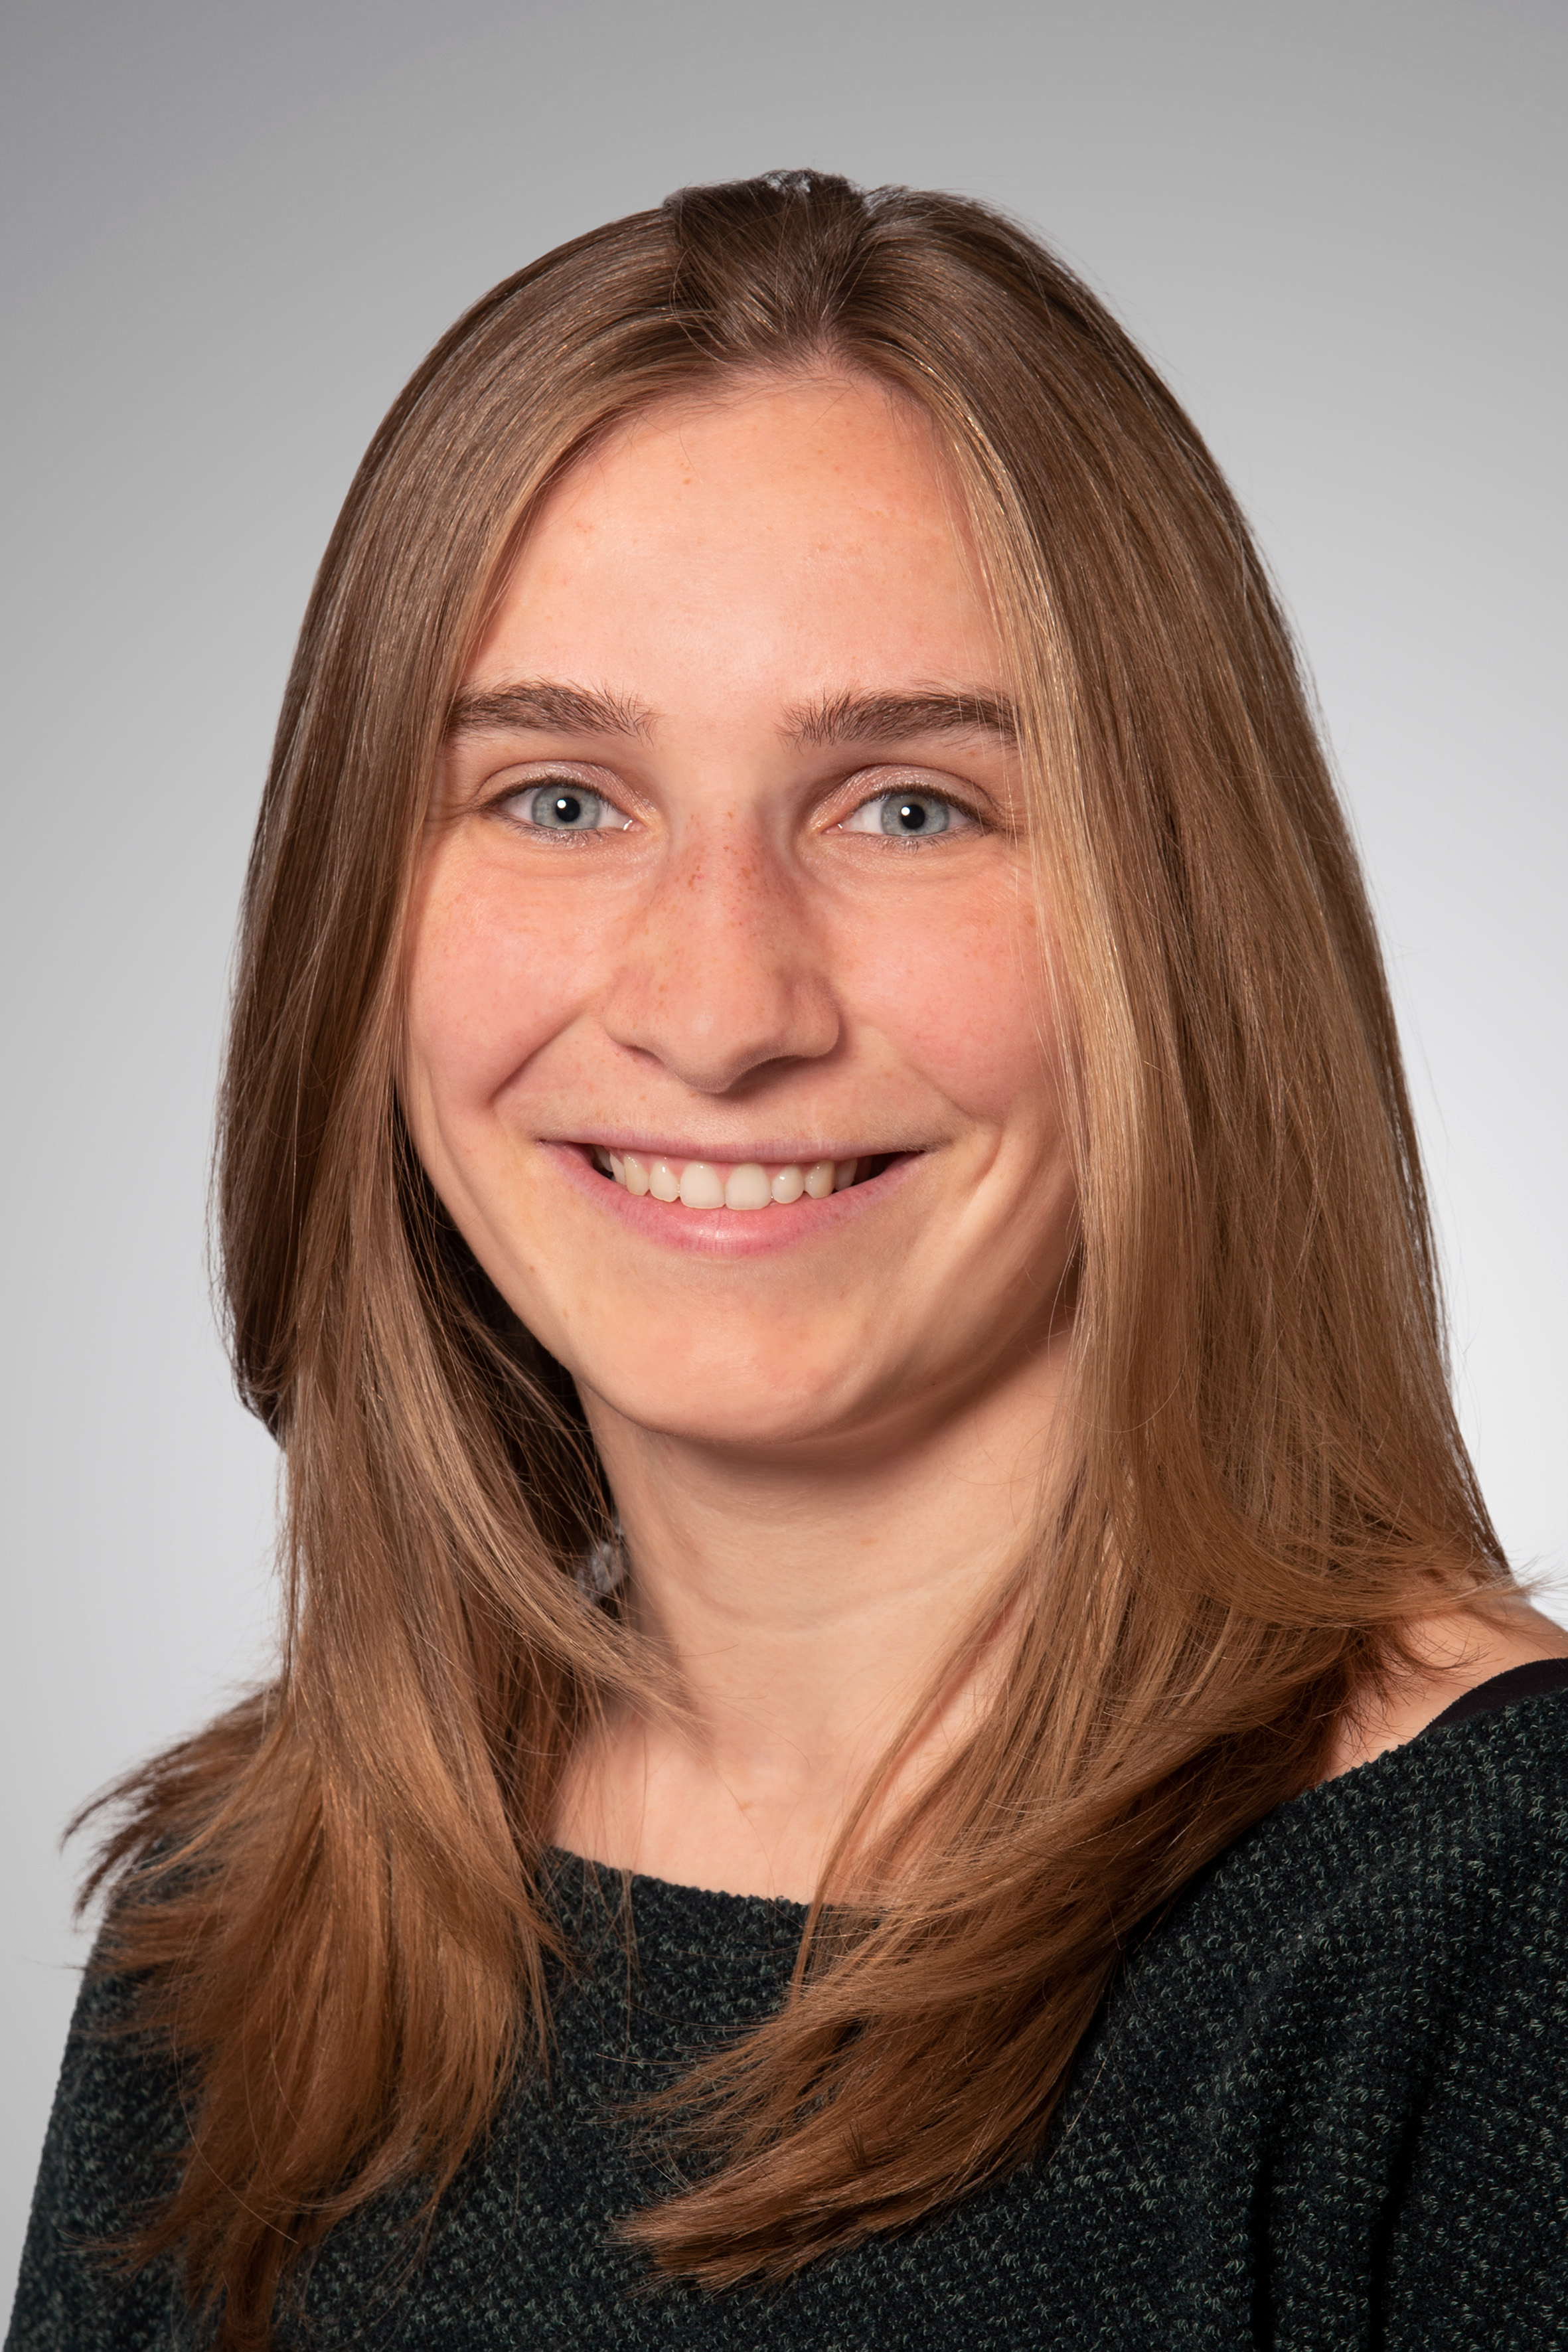
\includegraphics[width=\linewidth]{../resources/Profile_Picture.jpg}%	%trimming relative to image size

%---------------------------------------------------------------------------------------
%	META SKILLS
%----------------------------------------------------------------------------------------
  \fcolorbox{white}{white}{\begin{minipage}[c][1.5cm][c]{1\mpwidth}
    \LARGE{\textbf{\textcolor{darkcol}{Pauline Hasler}}} \\[2pt]
    \normalsize{ \textcolor{maincol} {Embedded Software Engineer} 
        \vspace{10pt}}
  \end{minipage}}

\renewcommand{\cvsection}[1]{
   \scalebox{0.95}[1]{\LARGE\bfseries \textcolor{darkcol}{#1}}

  \vspace{+5pt}
}




\cvsection{Contact}
\vspace{5pt}
\icontext{map-marker}{8mm}{Bungertenstrasse 12\\8307 Effretikon}{black}{lightaccentcol}\\[8pt]
\icontext{mobile}{8mm}{+41 78 695 64 19}{black}{lightaccentcol}\\[8pt]
\iconemail{envelope}{8mm}{pa.hasler@protonmail.com}{pa.hasler@protonmail.com}{black}{lightaccentcol}\\[8pt]
% \iconhref{github}{8mm}{github.com/hasler100}{https://github.com/Hasler100}{black}{lightaccentcol}\\[8pt]
\iconhref{linkedin}{8mm}{linkedin.com/pauline-hasler}{https://www.linkedin.com/in/pauline-hasler}{black}{lightaccentcol}\\

\vspace{+5pt}

\cvsection{Programming}
\cvsection{Languages}
    \cvskill{C} {Very good} {0.8} \\[-3pt]
    \cvskill{C++} {Beginner} {0.2} \\[-3pt]
    \cvskill{Python} {Basic knowledge} {0.4} \\[-3pt]
\cvsection{Operating Systems}
    %\cvskill{Freertos} {Very good} {0.8} \\[-2pt]
    \cvskill{Zephyr} {Good} {0.6} \\[-3pt]
    \cvskill{Yocto}{Beginner} {0.2} \\[-3pt]
    \cvskill{ROS}{Beginner} {0.2} \\[-3pt]
    \cvskill{Linux/Windows} {Basic knowledge} {0.4} \\[-3pt]
\cvsection{Tools}
    \cvskill{GitLab} {Good} {0.4} \\[-3pt]
    %\cvskill{Jenkins} {Basic knowledge} {0.4} \\[-3pt]
    \cvskill{Docker} {Basic knowledge} {0.4} \\[-3pt]
    %\cvskill{SVN} {Good} {0.6} \\[-3pt]

\newpage
\cvsection{\\}
\cvsection{Language Skills}
{  \vspace{-4pt}(Dyslexic)\\[6pt] }
    \cvskill{German} {Excellent} {1} \\[-3pt] 
    \cvskill{English} {Good} {0.7} \\[3pt]
\cvsection{Social Skills}
    \icontext{caret-right}{4mm}{Team player}{black}{accentcol}\\[6pt]
    \icontext{caret-right}{4mm}{Solution-oriented}{black}{accentcol}\\[6pt]
    \icontext{caret-right}{4mm}{hands-on}{black}{accentcol}\\[6pt]
    \icontext{caret-right}{4mm}{Communicative}{black}{accentcol}\\[6pt]

\cvsection{Additional Skills}
    \icontext{caret-right}{4mm}{Visual Studio Code}{black}{accentcol}\\[6pt]
    %\icontext{caret-right}{4mm}{Driving license category B1}{black}{accentcol}\\[6pt]
    \icontext{caret-right}{4mm}{Freertos}{black}{accentcol}\\[6pt]
    \icontext{caret-right}{4mm}{Jenkins}{black}{accentcol}\\[6pt]
    \icontext{caret-right}{4mm}{SVN}{black}{accentcol}\\[6pt]
    %\icontext{caret-right}{4mm}{Docker}{black}{accentcol}\\[6pt]
    %\icontext{caret-right}{4mm}{Polarion}{black}{accentcol}\\[6pt]
    \icontext{caret-right}{4mm}{CAD: Autodesk Inventor}{black}{accentcol}\\[6pt]

% hofixes to create fake-space to ensure the whole height is used

\renewcommand*\familydefault{\sfdefault}

\vspace{10pt}
\cvsection{Hobbies and Interests}
    \icontext{caret-right}{4mm}{Bouldering}{black}{accentcol}\\[6pt]
    \icontext{caret-right}{4mm}{Small projects}{black}{accentcol}\\[6pt]
    \icontext{caret-right}{4mm}{Drawing}{black}{accentcol}\\[6pt]


%\cvqrcode{0.3}

\end{leftcolumn}
\begin{rightcolumn}

%---------------------------------------------------------------------------------------
%	PROFILE
%----------------------------------------------------------------------------------------
\cvsection{Profile}

\cvtext{I studied Systems Engineering at ZHAW with a focus on Mechatronics. During my studies, I discovered my passion for embedded software development. Since January 2022, I have been working as an Embedded Software Engineer at Baumer Group, where I developed several sensor firmwares in C and actively contributed to the further development of the framework. I particularly appreciate the opportunity to use new technologies 
%such as Zephyr RTOS 
and the close collaboration within the team.}

%---------------------------------------------------------------------------------------
%	EDUCATION
%----------------------------------------------------------------------------------------
\cvsection{Education}

\cvevent
    {09.2018 - 07.2021}
    {Bachelor of Science ZHF in Systems Engineering}
  {ZHAW Winterthur}
  {Specialization: Mechatronics \\ Bachelor thesis: Multi-Level-TOF\\ Electives: Microcomputer Systems, Sensor Technology, Digital Signal Processing}

\cvevent
    {08.2017 - 07.2018}
    {Vocational Baccalaureate 2}
    {Vocational School lkj, focus: Technology}{}

%---------------------------------------------------------------------------------------
%	Berufserfahrung
%----------------------------------------------------------------------------------------

\cvsection{Work Experience}

\cvevent
    {01.2022 -- present}
    {Embedded Software Engineer}
  {Baumer Group: Firmware development for sensors}
  {Responsibilities: Development of sensor firmware and framework, especially with C and Zephyr RTOS. Further development of automated test procedures as well as close teamwork.}

\cvevent
    {07.2016 -- 08.2017}
    {Design Engineer}
  {ELEX AG: Design / Project Management}
  {Responsibilities: Design of customer-specific electrostatic precipitators. Coordination of subprojects with subsidiaries.}

%---------------------------------------------------------------------------------------
%	Projekte und Praktika
%----------------------------------------------------------------------------------------


\cvsection{Projects and Internships}

\cvtext{The list of projects and internships is not exhaustive. Further activities as an Embedded Software Engineer are listed in the interim reference from Baumer Group. \\ }
  
\cvevent{}{OM60: Triangulation Sensor}
    {Tools: Python, Anaconda, C, GitHub}
    {The OM60 is a high-precision triangulation sensor and the first sensor at Baumer Frauenfeld to use the new sensor framework. As part of this pilot project, which was implemented using agile methods, I took over the lead in firmware development. I was responsible for the sensor architecture, focusing on robust firmware with real-time requirements and reliable data communication.}

\cvevent{}{Application Template}
    {Tools: Python, Anaconda, C, GitHub\\Grade: 5, team of 2}
    {Based on the OM60 firmware, the Application Template was developed. The goal was to create a basis for further sensor projects that covers the common interfaces and functionalities of Baumer sensors. The entire framework team worked together on the optimal implementation. Modularity and code size were particularly important.}

\cvevent{}{Bachelor thesis: Multi-Level-ToF}
    {Tools: Python, Anaconda, C, GitHub\\Grade: 5, team of 2}
    {In this thesis, the resolution of a time-of-flight camera was improved by capturing images at different frequencies and combining them into one image. First, two concepts were defined, then the measurement range of the camera was determined and measured. The data obtained was evaluated with a program and the expected improvement in resolution was simulated. Afterwards, the new measurement methods were implemented, measured, and compared with the expected data. In addition, an attempt was made to optimize the new measurement method and integrate it directly into the camera firmware.}
    \vfill\null

\cvevent{}{Project work: Flexible Joint}
    {Tools: Python, ROS, GitHub\\Grade: 5.5, team of 2}
    {This is a statically indeterminate joint that can be controlled to different positions by compressed air. For a given chamber pressure and an applied force, the angle was measured. This was repeated for a defined measurement range. Based on this data, the force was determined for a given chamber pressure and angle. Finally, force feedback was implemented so that a certain force (e.g., a blow) triggers a reaction (e.g., the joint relaxing).}

\cvevent{}{Internship work: Microcontrollers}
    {Tools: C, Keil uVision, Ubuntu, Yocto Project, SVN}
    {Internships on: Edge detection, power management, control of a motion sensor (DMA and file system handling), programming an egg timer (creating a custom scheduler, working with state machines, GPIO, etc.)\hfill\break On embedded Linux: First steps with Yocto, creating a kernel module, handwriting recognition, embedded machine learning, scheduling, controlling GPIOs.}
  
\cvevent{}{Internship work: Computer Engineering}
    {Tools: Assembly, C, Keil uVision}
    {Controlling switches and lamps with memory maps, addition and multiplication considering flags, handling interrupts, saving and restoring register values in subroutines, working with timers, ADC, GPIO, UART and SPI, creating finite state machines.}
  
\cvevent{}{Internship work: Other}
    {Tools: C++, Matlab, Simulink, Mbed, Assembly, GitHub, SVN, etc. }
    {The systems engineering curriculum is extremely diverse, as computer science, mechanics, and electronics are taught. A special feature at ZHAW is the internship-accompanied teaching, through which I was able to gain many more practical experiences. These include, among others: \\
    Balancing a cube on an edge using a flywheel, controlling a ball-beam system, a water level, or other systems (control engineering), \\
    Creating spectrograms, filtering digital and analog signals, adding and filtering sound on audio recordings (digital signal processing), \\
    Measuring and analyzing the behavior of various sensors (sensor technology), \\
    Programming industrial and mobile robots, creating maps using a gyroscope (robotics).}


%---------------------------------------------------------------------------------------
%	Publikationen
%----------------------------------------------------------------------------------------
%\cvsection{Publikationen}

%---------------------------------------------------------------------------------------
%	Referenzen
%----------------------------------------------------------------------------------------

\cvsection{References}

\cvtext{References available upon request.\\ }


\vspace{2.5cm}


Effretikon, \today     \hspace{1cm}  % \hrulefill


\hspace*{30mm}\phantom{Effretikon, \today }

\end{rightcolumn}
\end{paracol}

\end{document}
